\section{Reviewer controls: state matching and interpretation}
These diagnostics were registered after the final confirmation, without changing any encoder, relation operator, or readout. We separately report previously inspected tests and a new set of 128 complete orbits (64 IID inputs and 32 collision pairs). The new orbits exclude training and validation of all five sources and every previously inspected test orbit. This is a small post-confirmation replication, not a new five-dataset study.

\paragraph{Predicted-state replication and distribution controls.}
On new collision pairs, the linear recipient reaches 10.00\%; correct predicted-null transfer reaches 15.31\%, versus 7.19\% for incorrect transfer. The difference is 8.125 points, with a descriptive crossed source/pair interval [1.25,15.625]; all five source differences are positive.
Validation-fitted mean/covariance transport of the incorrect donor reaches 7.50\%. This control addresses marginal null-coordinate distribution, not conditional state error, row/null dependence, or complete manifold membership.
Nearest-reference RMS distance is 0.565 for the correct hybrid, 0.616 for the incorrect hybrid, and 0.388 for true intermediate states. These distances concern natural training intermediates; they do not constitute a manifold-membership test. The distribution-shift explanation remains unresolved.

\paragraph{Error matching and its limitations.}
Within-input restriction to original correct/incorrect predictions whose null norms and errors both agree within 10\% retains only 3 source--sample observations; a 25\% restriction retains 18 of 320. The latter conditional difference is $-5.56$ points and is too sparse to support a stable mechanism conclusion. Conditioning on prediction error can remove a pathway through which correspondence acts; this is descriptive, not causal isolation.
An additional oracle diagnostic exactly matches each correct hybrid's null norm and error to the true intermediate, while preserving its row component. Reorienting a wrong donor yields 34.69\%, and randomized orientations yield 70.47\%. These controls use the true intermediate's direction. They are not learned predictions or evidence that wrong-pair training generalizes better. Their scope is narrower: equal scalar state error and norm do not imply equal downstream utility. Norm/error and marginal covariance controls are separate, rather than simultaneously matching all distributions.

\paragraph{Answers remain decodable from the null space.}
Independent ridge probes use support labels and known validation for regularization selection; they never update the composition pipeline. On true intermediate null coordinates, fresh-collision current-answer accuracy is 54.06\% (training-mode baseline 8.13\%) and future-answer accuracy is 52.81\%. Future labels are supplied only to these diagnostic probes. Thus the null component is invisible to one fixed linear readout, but is not independent of answer information.

\paragraph{Numerical audit.}
All five $13\times128$ readouts have numerical rank 13. SVD and pseudoinverse projectors agree; across every tested intervention and random draw, the maximum first-logit change is $4.11\times10^{-13}$. Norm/error matching discrepancies are below $1.14\times10^{-13}$. Independent reconstruction checks 499,530 sample/identity entries. These checks validate the defined interventions, not a natural relation-specific causal mechanism.

\begin{figure}[t]
\centering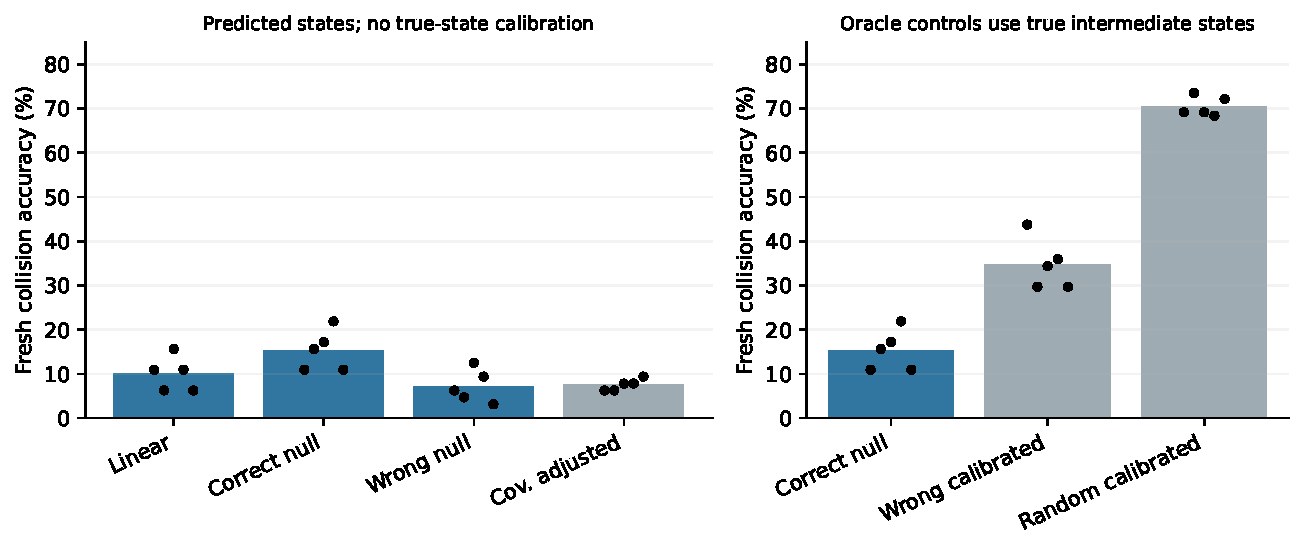
\includegraphics[width=\linewidth]{figures/reviewer_controls.pdf}
\caption{Frozen-model reviewer controls on new collision pairs. Dots show five source initializations, sharing test inputs. Right-hand calibrated controls use true intermediate states and are diagnostics only; they are not available predictors.}
\end{figure}
